\section{Setup}
\label{sec:setup}

\subsection{Model, sampling and recording}
\label{sec:models}
We study MDM \citep{tevet2023mdm}, a kinematic diffusion model: a transformer encoder (8 layers, width 512) with a CLIP text encoder, using two official HumanML3D checkpoints: the 50-step model and the original 1000-step model. Both generate 120 frames (6\,s at 20\,fps) in the HumanML3D representation \citep{guo2022humanml3d}, with classifier-free guidance at scale 2.5. At six denoising steps, evenly spaced from the first to the last, we record the output of every transformer layer at every fourth frame (dropping the condition token), the noisy input $\vx_t$, and the model's clean-motion estimate $\hat\vx_0$ with its decoded joints. Guidance runs a conditional and an unconditional pass; we record the activations of the conditional pass and the guided estimate that the sampler uses. ``20\% of denoising'' denotes the second recorded step (step 10 of 50, or 200 of 1000). Figure~\ref{fig:setup} summarizes what we record and compare.

\begin{figure}[t]
\centering
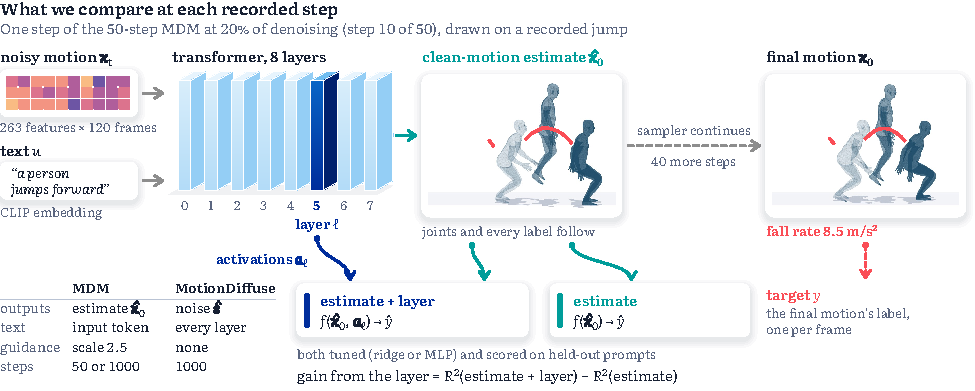
\includegraphics[width=\linewidth]{figures/web/fig_setup.pdf}
\caption{What we compare, at one denoising step. The model receives the noisy motion $\vx_t$ and the text $u$; its layers produce activations $\va_\ell$, and its output gives the clean-motion estimate $\hat\vx_0$, from which joints and every label follow. Two readouts are trained to predict a label $y$ of the final motion $\vx_0$ (here the fall rate of a jump): one from the estimate alone (teal), one from the estimate and layer $\ell$ together (deep blue). The gain from the layer is the difference in their scores ($R^2$ or AUC), which for $R^2$ measures the conditional usable information (Proposition~\ref{prop:vinfo}). Drawn on a recorded jump of the 50-step MDM at 20\% of denoising: the estimate (center) already shows the jump of the final motion (right; center of mass red while airborne). Bottom left: where the two models differ (Section~\ref{sec:models}). The grid for the noisy input is schematic.}
\label{fig:setup}
\end{figure}

\paragraph{A second model.} To test whether the results depend on MDM's design, we repeat the main analyses on MotionDiffuse \citep{zhang2022motiondiffuse}, also kinematic but different where it matters. It predicts the noise rather than the clean motion, so its estimate $\hat\vx_0 = (\vx_t - \sqrt{1-\bar\alpha_t}\,\hat{\boldsymbol\epsilon})/\sqrt{\bar\alpha_t}$ is computed from its prediction and the noisy input; it uses no guidance; and its 8 transformer layers (width 512, linear attention, one token per frame) receive the text in every layer, through cross-attention and stylization blocks, rather than as a token. We use its official HumanML3D checkpoint and sampler (1000 DDPM steps), the same prompts, seeds, frames and recorded steps as for MDM (20\% of denoising is step 200), and choose its layers by the same rule as MDM's (Section~\ref{sec:fair}; layer 3 for balance, layer 6 for flight and gravity). Its noise schedule is linear where MDM's is cosine, so a given fraction of denoising is noisier for MotionDiffuse (Table~\ref{tab:snr}). Since the text reaches every layer, its estimate is a function of its activations, the noisy input and the text, $(\va_\ell, \vx_t, u)$ in the notation of Section~\ref{sec:fair}, so for this model the bound of Section~\ref{sec:fair} includes the text, which is one reason we also test the text directly.

\paragraph{Prompts and runs.} The prompt set combines 64 curated prompts (everyday locomotion, jumps and hops, balance-challenging actions, upper-body actions) with 186 captions sampled from the HumanML3D test split, 250 in total, and each prompt is sampled 4 times: 1,000 motions per run. We run each model with three seeds: 6,000 motions from the two MDM checkpoints and 3,000 from MotionDiffuse. Because few of these motions contain flight, we also run every model on a \emph{jump-heavy} prompt set with three seeds: the 14 curated jump, hop, leap and skip prompts plus one caption from every HumanML3D test motion whose caption names one of these actions, 245 distinct prompts sampled 4 times each (2,940 motions per model). A pilot used only the curated prompts (256 motions), every second frame, and a single held-out set of 12 prompts.

\subsection{Physical labels}
\label{sec:labels}
All labels are computed from joint positions, with $y$ the vertical axis, both for the final motion and for the clean-motion estimate at each recorded step.

\paragraph{Center of mass, contact and support.} The center of mass is $\vc_t = \sum_s m_s \tfrac12(\vp_{a(s),t} + \vp_{b(s),t})$, with standard segment mass fractions $m_s$ placed at segment midpoints, where $a(s)$ and $b(s)$ are the joints at the two ends of segment $s$ \citep{winter2009biomechanics}. An ankle (toe) joint is in contact when it is lower than 12\,cm (6\,cm) and moves less per frame than HumanML3D's contact threshold. The support region $S_t$ is the convex hull of the contacting foot joints on the ground plane, padded by 4\,cm.

\paragraph{Balance.} Dynamic balance uses the extrapolated center of mass \citep{hof2005condition},
\begin{equation}
    \vx^{\mathrm{XCoM}}_t = \vc^{xz}_t + \dot{\vc}^{xz}_t / \omega_0, \qquad \omega_0 = \sqrt{g/h}, \quad g = 9.81\,\mathrm{m/s^2},
\end{equation}
where $h$ is the motion's median center-of-mass height. The \emph{dynamic balance margin} is the signed distance from $\vx^{\mathrm{XCoM}}_t$ to the boundary of $S_t$, positive inside; the \emph{static balance margin} uses $\vc^{xz}_t$ instead. Both are undefined without foot contact. The extrapolated center of mass routinely leaves the support region during normal stepping, so we treat the margins as continuous quantities rather than failure labels (Figure~\ref{fig:labels}a,b). They are kinematic quantities; a test of physical feasibility would need the center of pressure or inverse dynamics.

\paragraph{Floating, flight and gravity.} The \emph{lowest-foot height} is the height of the lowest foot joint, and a frame is \emph{in flight} when no foot is in contact. A frame is \emph{airborne} when every foot joint is above its contact height and no knee, wrist or the pelvis is within 15\,cm of the floor, so that crawling and cartwheels do not count as airborne (Appendix~\ref{app:labelfix}). Over each airborne stretch of at least 0.2\,s we fit $c_y(t) = a_0 + a_1 t + a_2 t^2$ to the center-of-mass height. Ballistic flight requires the \emph{flight gravity} $\hat g = -2a_2$ to equal $g = 9.81\,\mathrm{m/s^2}$, a test that needs no calibration (Figure~\ref{fig:labels}c,d). Every frame of the stretch carries its $\hat g$. Because in the main data most airborne frames lie in stretches that barely fall (Section~\ref{sec:fairresults}), this flight gravity mixes two questions, and for probing we also split it at the floating cut-off below: whether an airborne frame belongs to a floating or a falling stretch (\emph{floats or falls}, scored by AUC), and the fitted gravity of falling stretches alone (the \emph{fall rate}).

\paragraph{Per-sample failures.} An airborne stretch with $\hat g < 2\,\mathrm{m/s^2}$ is \emph{floating}: the body is off the ground and unsupported, but barely falls. For each sample, the \emph{floating rate} is the share of frames in floating stretches, and the \emph{raised-contact rate} is the share of contact frames whose lowest foot is higher than 5\,cm. Two further per-sample rates serve only as inputs to the early-warning readouts (Section~\ref{sec:earlymethod}): the mean $|\hat g - g|$ over stretches that do fall, and the share of support frames with a negative dynamic balance margin.

\begin{figure}[t]
\centering
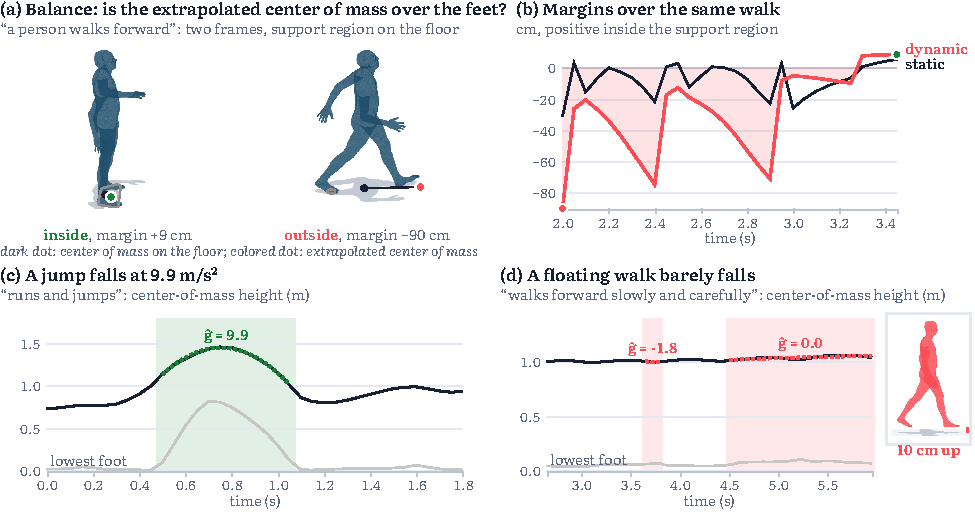
\includegraphics[width=\linewidth]{figures/web/fig_labels.pdf}
\caption{How the balance and gravity labels are computed, on recorded final motions of the 50-step model. (a) A walk at its most and least balanced frames: the support region on the floor (gray), the center of mass projected to the floor (dark dot) and the extrapolated center of mass (XCoM; green inside the support, red outside). (b) Over the same window, the dynamic margin is negative through most of each step. Dots mark the two frames in (a). (c) A jump: the parabola fitted to the center-of-mass height over the airborne stretch falls at close to 9.81\,m/s$^2$. (d) A floating walk: the body is unsupported, with the lowest foot 6 to 11\,cm up (median 9\,cm), but its center of mass barely falls, so $\hat g$ is below the 2\,m/s$^2$ cut-off; inset: one floating frame. Bodies are SMPL meshes fitted to the joints for display, as in Figure~\ref{fig:teaser}.}
\label{fig:labels}
\end{figure}

\subsection{What the model shows, and a fair comparison}
\label{sec:fair}
In our data, a linear probe on MDM's last layer predicts the final motion's dynamic balance better than the balance computed from the model's own estimate at the same step (Table~\ref{tab:naive}). It is tempting to conclude that the model knows how balanced the motion will be and fails to show it. But the estimate is computed from that layer, so everything it contains about balance has passed through the layer. The probe's advantage can mean only that the layer holds the information in a form a linear readout finds easy, while the estimate holds it in a form that needs a nonlinear readout or a computed quantity. To call the knowledge hidden, a readout of the layer has to beat an equally flexible readout of the estimate, or add to it. The rest of this section makes the argument precise.

At each step the model shows its clean-motion estimate $\hat\vx_0^{(k)}$: 263 features per frame, from which joints and every label above follow exactly. We number MDM's encoder layers 0 to 7. Each layer's output is a deterministic function of the previous layer's, and the output of layer 7, the last, is mapped to the conditional estimate by a fixed linear projection at every frame. Guidance combines this conditional estimate with an unconditional one, which depends only on $\vx_t$ and the step. Write $\va_\ell^{(k)}$ for the full conditional output of layer $\ell$ at step $k$ (every token, including the condition token), $\vx_t$ for that step's noisy input, and $u$ for the text condition. The guided estimate is then a function of $(\va_\ell^{(k)}, \vx_t)$ for every $\ell$, and the activations are a function of $(\vx_t, u)$. For any label $y$ of the final motion, the data-processing inequality therefore gives
\begin{equation}
    I\big(y;\, \hat\vx_0^{(k)}\big) \;\le\; I\big(y;\, \va_\ell^{(k)}, \vx_t\big) \;\le\; I\big(y;\, \vx_t, u\big).
\end{equation}
The estimate cannot carry information about the outcome that the activations and the noisy input lack. The same argument bounds the video studies of Section~\ref{sec:related} from the other side: under forward noising the activations are functions of the clean latent, the text prompt and noise drawn independently of both and of the label, and under deterministic inversion they are functions of the clean latent and the prompt alone, so no layer can carry more information about the label than the clean latent together with the prompt.

Shannon information therefore cannot separate these representations. What differs is how much of the information a given readout can use. For a family $\mathcal V$ of readouts, the $\mathcal V$-information $I_{\mathcal V}(X \to y)$ is the reduction in the best expected loss on $y$ that a readout in $\mathcal V$ achieves by seeing $X$ \citep{xu2020vinfo}. Unlike Shannon information, it can grow under processing, which is how a probe on the layer can beat a readout of the estimate. The question that bears on hidden knowledge is what the layer adds to the estimate \citep{hewitt2021conditional},
\begin{equation}
    I_{\mathcal V}\big(\va_\ell^{(k)} \to y \mid \hat\vx_0^{(k)}\big) \;=\; H_{\mathcal V}\big(y \mid \hat\vx_0^{(k)}\big) - H_{\mathcal V}\big(y \mid \hat\vx_0^{(k)}, \va_\ell^{(k)}\big),
\end{equation}
which we measure as the gain in $R^2$ (or AUC) from adding the layer to a readout of the estimate. For squared-error readouts, once the baseline $R^2$ is fixed, the two determine each other:
\begin{proposition}\label{prop:vinfo}
Let $\mathcal V$ predict Gaussians $\mathcal N(f(\cdot), \sigma^2)$, with $f$ from a regression class and $\sigma > 0$ free, and let the class on $(\hat\vx_0^{(k)}, \va_\ell^{(k)})$ contain every function in the class on $\hat\vx_0^{(k)}$. Writing $R^2_X$ for the best $R^2$ the class reaches from $X$,
\begin{equation}
    I_{\mathcal V}\big(\va_\ell^{(k)} \to y \mid \hat\vx_0^{(k)}\big) \;=\; \tfrac12 \log \frac{1 - R^2_{\hat\vx_0^{(k)}}}{1 - R^2_{\hat\vx_0^{(k)}, \va_\ell^{(k)}}} \;\ge\; 0 .
\end{equation}
\end{proposition}
For a fixed baseline, the gain in $R^2$ is therefore a monotone transform of the conditional usable information (proof in Appendix~\ref{app:proofs}), and in population it cannot be negative: a negative measured gain only reflects fitting the larger readout on finite data. Its value depends on the family, so we report it for linear readouts, a fixed MLP and readouts tuned on held-out prompts, test whether it survives within a prompt, and vary the amount of training data. Our per-frame probes see only the conditional pass, without the condition token, and one recorded frame at a time, so strictly they could see less than the estimate. On the 50-step model, adding the condition token gains at most 0.004 for balance, flight and floating (Appendix~\ref{app:impl}).

\paragraph{Readouts.} For each label and recorded step we compare six readouts, each predicting the final motion's per-frame label:
\begin{itemize}
    \item \textbf{Explicit}: the same label computed from the estimate's joints, with a linear calibration fit on the training folds (for the flight AUC, the raw value);
    \item \textbf{Estimate, linear}: a ridge probe on the estimate's 263 features, the usual baseline in probing studies;
    \item \textbf{Estimate, MLP}: a small MLP on everything the estimate shows, that is its 263 features plus the labels computed from it (Section~\ref{sec:labels}, with foot contacts and foot sliding speed) and indicators for undefined values;
    \item \textbf{Layer, linear} and \textbf{Layer, MLP}: ridge and the same MLP on one layer's 512 activations at the frame (its slice of $\va_\ell$);
    \item \textbf{Estimate + layer, MLP}: the same MLP on both, which asks whether the layer adds anything to what the estimate shows.
\end{itemize}
We also report a ridge probe on the noisy input $\vx_t$. Ridge probes standardize their inputs and choose the penalty from $\{1, 10, \dots, 10^4\}$ by efficient leave-one-out cross-validation on the training frames. The MLP has two hidden layers of 256 units with ReLU and dropout 0.1, and is trained with AdamW (learning rate $10^{-3}$, weight decay $10^{-4}$) with early stopping on 15\% of the training prompts. The layer is fixed per label as the one with the best mean linear score at 20\% of denoising: layer 7 for both balance measures, 6 for flight, and 5 for gravity and its two parts, on both MDM checkpoints. This choice favors the layer in a standalone comparison; for what the layer adds to the estimate, we also test every layer and all layers together (Section~\ref{sec:fairresults}).

\paragraph{Tuned readouts on pooled seeds.} The fixed MLP and the leave-one-out penalty (which validates on frames of motions seen in training) could each favor one side. We therefore repeat the comparison with every run of a checkpoint pooled, three seeds and 3,000 motions, under five folds grouped by prompt across seeds, and with every readout tuned on a validation split of 15\% of the training prompts. The families are ridge, with the penalty chosen from $10^{-1}$ to $10^{6}$; an MLP family that adds a linear map to an MLP, so that it contains the linear readout, with five configurations (64 to 1024 hidden units, one or two hidden layers, dropout 0.1 or 0.3, weight decay $10^{-4}$ to $10^{-2}$); and, as the \emph{tuned} readout, whichever of the two has the lower validation error. The same procedure reads the estimate's 263 raw features alone, everything the estimate shows, the layer, and estimate and layer together. The conditional gain uses a readout of estimate and layer that may fall back to the estimate alone: among the candidates for both inputs and for the estimate alone, it keeps the one with the lowest validation error, so that the larger input cannot lower the score merely by being harder to fit. Confidence intervals resample prompts with replacement (1,000 replicates, the same draw for every readout). They do not include training variance, which we measure by refitting with two further validation splits and initializations. We report many intervals (targets, models, layers and steps) without correcting for multiplicity, read them as descriptive, and draw conclusions only from patterns that hold across models, layers and scores. The analysis was not preregistered: the tuned readouts, the jump-heavy runs, the split of flight gravity and the second model were added after the first results (Appendix~\ref{app:fixedmlp}).

\paragraph{Evaluation.} All readouts share five folds grouped by prompt, so no test prompt is seen in training. We report $R^2$ for continuous labels and ROC-AUC for flight and for floats or falls, pooled over all test frames. Since physics differs greatly between prompts, a readout could score well by recognizing the prompt alone. The \emph{within-prompt} score removes that possibility: we subtract each prompt's mean from both target and prediction and report the Pearson correlation of the residuals, which only sample-specific information can raise. A prompt also says when things tend to happen (a jump in the middle of the clip, say), which a per-frame readout could exploit within a prompt. With seeds pooled, the \emph{within-prompt-and-frame} score removes this as well, by subtracting the mean over the 12 samples of the same prompt at the same frame. The within-prompt score cannot be raised by information that enters a prediction additively through the prompt, and the within-prompt-and-frame score by information that enters additively through the prompt and the frame:
\begin{proposition}\label{prop:within}
If a prediction has the form $\hat y = f(X) + h(c)$, with $X$ the readout's input, where $h$ depends only on the cell $c$ (the prompt, or the prompt and the frame), then its within-cell score equals that of $f(X)$.
\end{proposition}
A gain within prompt and frame is therefore information beyond anything the text and the timing of a prompt could add on their own (proof in Appendix~\ref{app:proofs}); interactions between the text and the estimate are tested separately, by giving the readout the text itself (Section~\ref{sec:fairresults}). To see how the comparison depends on data, we also retrain the linear layer probe and the explicit calibration on random subsets of 13 to all ($\approx$200) training prompts per fold, and the tuned readouts with seeds pooled on subsets of 25, 50 and 100, and evaluate on the same test folds.

\subsection{Early warning}
\label{sec:earlymethod}
Can a sample that will float be caught partway through sampling and replaced? A sample fails if its final motion has any floating. We compare four strategies and count cost in denoising steps per delivered motion (1 = one full sample): generating once; \emph{finish, then filter}, which checks the final motion and regenerates if it floats; \emph{early abort}, which scores the sample at 20\% or 40\% of denoising and restarts it if the score is high; and early abort followed by the final check. Retries stop after a budget of attempts, and the last attempt is always delivered. The early score is (i) a training-free rule, abort if the decoded estimate already shows floating; (ii) a ridge readout, trained out of fold and set to abort the same share of samples, of everything the estimate shows (its features averaged over frames and its per-sample failure rates), of the frame-averaged activations of one layer (layer 3 of the 50-step model and layer 6 of the 1000-step model, each chosen on the first seed), or of both; (iii) random aborts at the same rate; or (iv) a perfect detector, as a ceiling. All strategies are simulated with the same random draws, on the 6,000 recorded MDM samples. Each already contains its estimate at every recorded step and its final motion, so every decision uses what an online run would see; a retry draws another recorded sample of the same prompt (200 simulated requests per prompt). Strategies that end with the final check are compared at equal delivered failure by varying the budget from 1 to 20 attempts.
